\PassOptionsToPackage{unicode}{hyperref}
\PassOptionsToPackage{naturalnames}{hyperref}
\documentclass{article}
\usepackage{geometry}
%\usepackage{fullpage}
\usepackage{parskip}
\usepackage{physics}
\usepackage{amsmath}
\usepackage{amssymb}
\usepackage{xcolor}
\usepackage[colorlinks,linkcolor=blue,citecolor=green]{hyperref}
\usepackage{array}
\usepackage{longtable}
\usepackage{multirow}
\usepackage{comment}
\usepackage{graphicx}
\usepackage{cite}
\usepackage{amsfonts}
\usepackage{bm}
\usepackage{slashed}
\usepackage{dsfont}
\usepackage{mathtools}
\usepackage[compat=1.1.0]{tikz-feynman}
\usepackage{simplewick}
%\usepackage{fourier}
%\usepackage{slashbox}
%\usepackage{intent}
\usepackage{mathrsfs}
\usepackage{xparse}
\usepackage{enumerate}
\usepackage{listings}
\usepackage{gensymb}

\geometry{left=0.9cm,right=0.9cm,top=1.5cm,bottom=2cm}

\newcommand{\gm}{\gamma^{\mu}}
\newcommand{\gn}{\gamma^{\nu}}
\newcommand{\gs}{\gamma^{\sigma}}
\newcommand{\gr}{\gamma^{\rho}}
\newcommand{\gnr}{g^{\nu\rho}}
\newcommand{\gmr}{g^{\mu\rho}}
\newcommand{\gms}{g^{\mu\sigma}}
\newcommand{\gns}{g^{\nu\sigma}}
\newcommand{\vbp}{\vb{p}}
\newcommand{\vbk}{\vb{k}}
\newcommand{\g}{\gamma}
\renewcommand{\a}{\alpha}
\renewcommand{\b}{\beta}
\renewcommand{\t}{\theta}
\newcommand{\la}{\lambda}
\newcommand{\p}{\phi}
\newcommand{\vp}{\varphi}
\newcommand{\s}{\sigma}
\renewcommand{\G}{\Gamma}
\newcommand{\pars}{\slashed\partial}
\newcommand{\ps}{\slashed p}
\newcommand{\ks}{\slashed k}
\newcommand{\bP}{\vb{P}}
\newcommand{\bA}{\vb{A}}
\newcommand{\ba}{\boldsymbol{\alpha}}
\newcommand{\apo}{\abs{\vb{p}_1}}
\newcommand{\aps}{\abs{\vb{p}_2}}
\newcommand{\lag}{\mathcal{L}}

\definecolor{mygray}{rgb}{0.9,0.9,0.9}
\lstset{
  frame=single,
  backgroundcolor=\color{mygray},
  extendedchars=true,
  language=Mathematica
}

\title{Hadron Spectroscopy}
\author{Yingsheng Huang}
\begin{document}
\maketitle

\begin{enumerate}
  \item Prove Landau-Yang theorem.

	For any vector particles,we can always write the field operator as a single vector field.
  $$A_{\mu}(x)=\int\frac{\dd^3k}{(2\pi)^3}\frac{1}{\sqrt{2\abs{\vb{k}}}}\sum_{\la}(a^{\la}_{\vbk}\epsilon^{\la}_{\mu}(k)e^{-ik\cdot x}+{a^{\la}_{\vbk}}^{\dagger}{\epsilon^{\la}_{\mu}}^*(k)e^{ik\cdot x})$$
  Then the feynman rules can be easily derived. The amplitude of $vector\rightarrow \g\g$ is
  \begin{align*}
    i\mathcal{M}&=\epsilon_1^{*\mu}(p_1)\epsilon_2^{*\nu}(p_2)\epsilon^{\a}(p)\Gamma_{\mu\nu\s}\\
    \intertext{since it must obey Lorentz-invariant}
    &=(\epsilon_1\cdot\epsilon_2)(a_1\epsilon\cdot p_1+a_2\epsilon\cdot p_2)+a_3(\epsilon_1\cdot \epsilon)(\epsilon_2\cdot p_1)+a_4(\epsilon_2\cdot \epsilon)(\epsilon_1\cdot p_2)\\
    \intertext{final states symmetry (identical), $a_1=a_2$, first term vanishes. And $\epsilon_2\cdot p_1=\epsilon_1\cdot p_2=0$}
    &=0
  \end{align*}
  \item $\eta\rightarrow\pi\pi$

  For $\eta$ meson, $I^GJ^{PC}=0^+0^{-+}$, for $\pi$ meson, $I^GJ^{PC}=1^-0^{-+}$. Charge parity conservation gives the final state angular momentum must be even, so $\pi\pi$ system gives positive parity, parity is not conserved. (For $\pi^0\pi^0$ system, use identical particle instead.)

  \item $\eta\rightarrow\pi\pi\pi$

	From previous discussion, we know that this reaction can happen not only under weak interaction for $P$ parity and $C$ parity are conserved. But $G$ parity is not conserved, the final state $G$ parity is negative while the initial state is positive, so it must not be a strong interaction.

	\item $\rho\rightarrow\pi\pi$

	  For $\rho$ meson, $I^GJ^{PC}=1^+1^{--}$. For angular momentum conservation, the final state orbital angular momentum must be $L=1$ while the spin $S$ is zero. For $\pi^0\pi^0$ scenario, $L+S=even$ is not guaranteed. For $\pi^+\pi^-$ scenario, $CP=(-)^S=+$, no obvious violation, it can happen.

	  \item $\omega\rightarrow\pi^0\pi^0\pi^0$

		For $\omega$ meson, $I^GJ^{PC}=0^-1^{--}$. Apparently CP violation.

    \item Dalitz plot.
    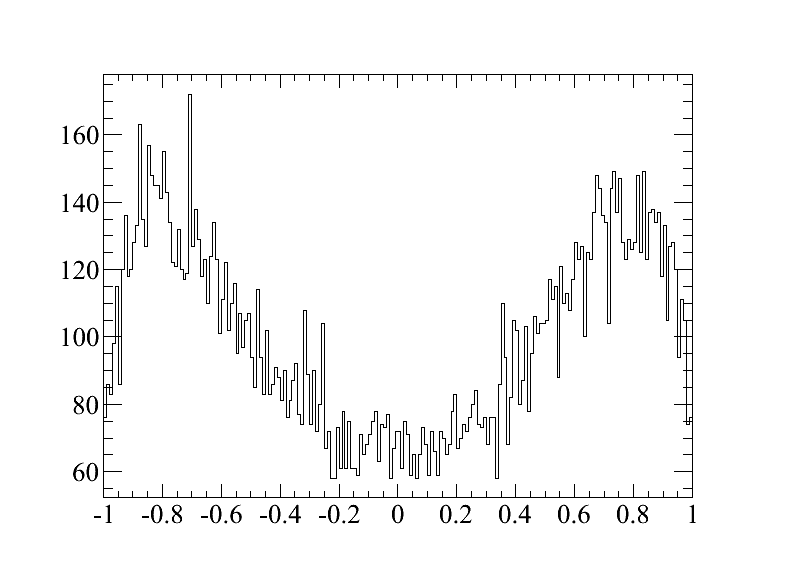
\includegraphics[width=4 in]{shenkeng.png}
    
    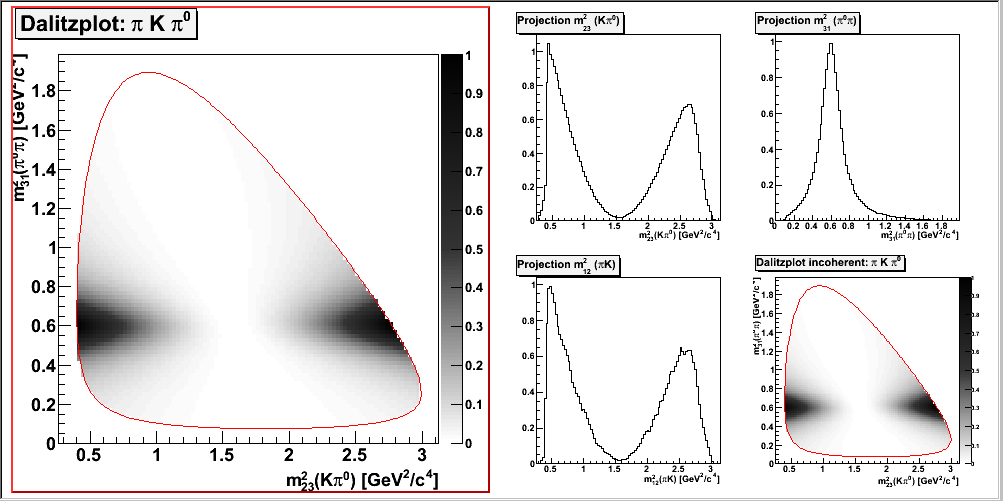
\includegraphics[width=4 in]{ss.png}
    \item $\eta-\eta'$ mixing.

    $$\eta_1=\frac{1}{\sqrt{3}}(u\bar u+d\bar d+s\bar s)$$
    $$\eta_8=\frac{1}{\sqrt{6}}(u\bar u+d\bar d-2s\bar s)$$
    and
    $$\pmqty{\eta\\\eta'}=\pmqty{\cos\theta_P&\sin\theta_P\\-\sin\theta_P&\cos\theta_P}\pmqty{\eta_1\\\eta_8}$$
    For $\eta$ and $\eta'$ to have the same $s\bar s$ and $(u\bar u+d\bar d)/\sqrt{2}$ contents, it must have $\tan\theta_P=\frac{1-\sqrt{2}}{1+\sqrt{2}}$, which leads to $\theta_P=9.7\degree$.

    $\omega-\phi$ mixing.

    $$\omega_1=\frac{1}{\sqrt{3}}(u\bar u+d\bar d+s\bar s)$$
    $$\omega_8=\frac{1}{\sqrt{6}}(u\bar u+d\bar d-2s\bar s)$$
    and
    $$\pmqty{\omega\\\phi}=\pmqty{\cos\theta&\sin\theta\\-\sin\theta&\cos\theta}\pmqty{\omega_1\\\omega_8}$$
    To have
    $$\omega=\frac{1}{\sqrt{2}}(u\bar u+d\bar d)$$
    $$\phi=s\bar s$$
    one must make $\frac{1}{\sqrt{3}}\cos\theta+\frac{2}{\sqrt{6}}\sin\theta=0$ and $-\frac{1}{\sqrt{3}}\sin\theta+\frac{1}{\sqrt{6}}\cos\theta=0$, which leads to $\tan\theta=\frac{1}{\sqrt{2}}$, $\theta=35.3\degree$.

\end{enumerate}
\end{document}
